\documentclass[a4paper, UKenglish]{lipics-v2018}

\usepackage[dvipsnames]{xcolor}

\usepackage[utf8]{inputenc}
\usepackage{graphicx}
\usepackage{amssymb}
\usepackage{amsfonts}
\usepackage{amsthm}
\usepackage{wrapfig}
\usepackage{makecell}
\usepackage{xspace}
\usepackage{caption}
\usepackage{wrapfig}
\usepackage{float}
\usepackage{MnSymbol}
\usepackage{todonotes}
\usepackage{chngpage}
\usepackage{multirow}
\usepackage{comment}

\newcommand{\myremark}[4]{\textcolor{blue}{\textsc{#1 #2:}} \textcolor{#4}{\textsf{#3}}}
\newcommand{\frank}[2][says]{\myremark{Frank}{#1}{#2}{SeaGreen}}
\newcommand{\patrick}[2][says]{\myremark{Patrick}{#1}{#2}{Plum}}
\newcommand{\maarten}[2][says]{\myremark{Maarten}{#1}{#2}{Red}}
\newcommand{\ivor}[2][says]{\myremark{Ivor}{#1}{#2}{Blue}}

\newtheorem{condition}{Condition}
\newtheorem{conjecture}{Conjecture}
\newtheorem{observation}{Observation}

\newcommand{\etal}{\textit{et al.}\xspace}

% macro for making mathcal definitions
\newcommand{\mkmcal}[1]{\ensuremath{\mathcal{#1}}\xspace}

% common mathcal definitions
\newcommand{\G}{\mkmcal{G}}
\newcommand{\Lst}{\mkmcal{L}}
\newcommand{\T}{\mkmcal{T}}
\newcommand{\C}{\mkmcal{C}}
\newcommand{\X}{\mkmcal{X}}
\newcommand{\D}{\mkmcal{D}}
\newcommand{\M}{\mkmcal{M}}
\newcommand{\E}{\mkmcal{E}}
\newcommand{\BB}{\mkmcal{B}}
\renewcommand{\S}{\mkmcal{S}}
\renewcommand{\H}{\mkmcal{H}}

\newcommand{\geod}{\pi\xspace}

% macro for mathbb definitons, for definiton of the naturals N, and booleans
\newcommand{\mkmbb}[1]{\ensuremath{\mathbb{#1}}\xspace}

\newcommand{\R}{\mkmbb{R}}

\def\polylog{\operatorname{polylog}}

\title{Trajectory Visibility in a Simple Polygon}
\titlerunning{Trajectory Visibility in a Simple Polygon}


\author{Patrick Eades}{University of Sydney}{patrick.eades@sydney.edu.au}{}{}
\author{Ivor van der Hoog}{Utrecht University}{i.d.vanderhoog@uu.nl}{}{}
\author{Maarten Löffler}{Utrecht University}{m.loffler@uu.nl}{}{}
\author{Frank Staals}{Utrecht University}{f.staals@uu.nl}{}{}
\authorrunning{P. Eades, I. van der Hoog, M. L\"offler, and F. Staals}
\Copyright{Patrick Eades, Ivor van der Hoog, Maarten L\"offler, and Frank Staals}%mandatory, please use full first names. LIPIcs license is "CC-BY";  http://creativecommons.org/licenses/by/3.0/

\begin{document}

\maketitle

\vspace{-6.5cm}
\begin{wrapfigure}[0]{r}{0.6\linewidth}
    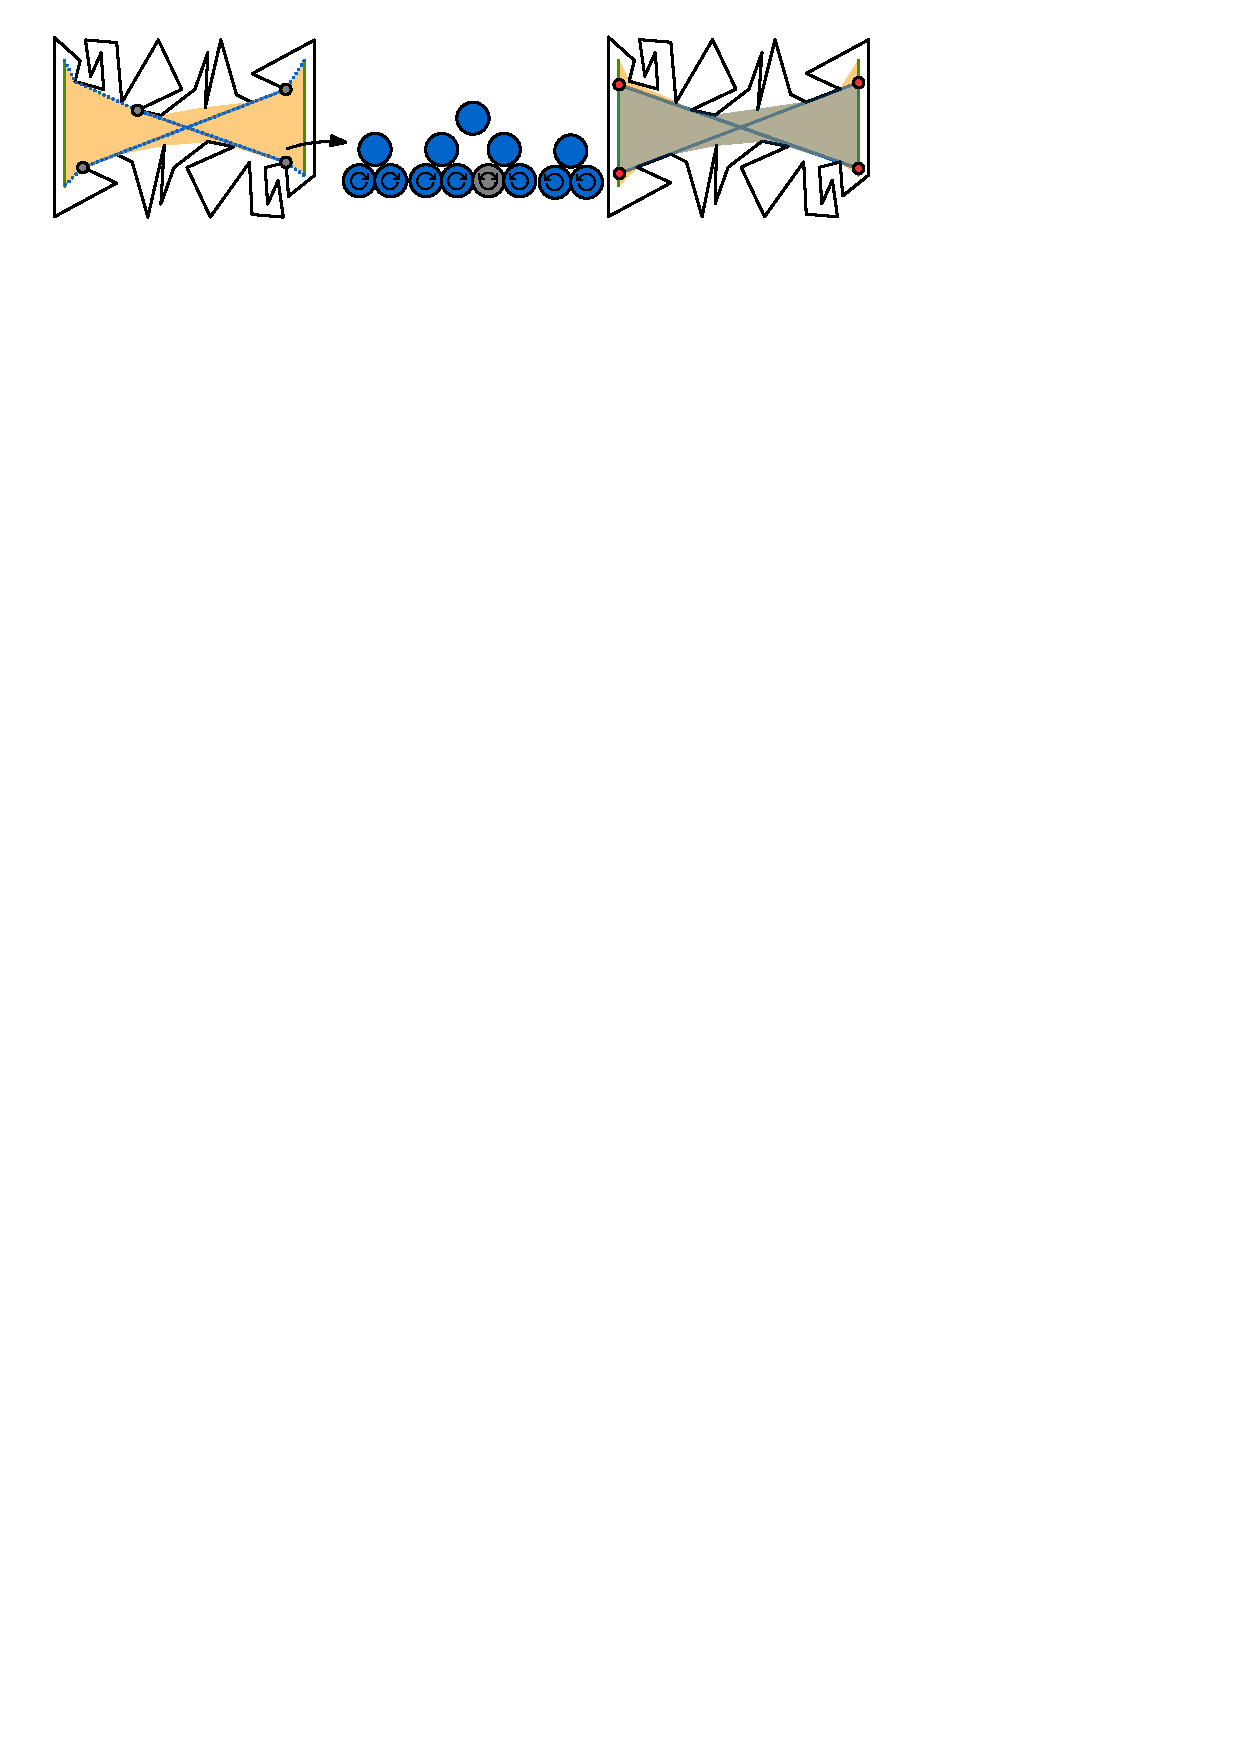
\includegraphics[width=8cm]{../visibilityglass}
    \centering
    \caption{(left) $H(e_1,e_2)$ in orange with the shortest paths between endpoints in dotted blue. The bitangents are underlined in grey. (middle) We obtain each dotted path as a collection of binary search trees, where only the bitangent starts in clockwise and ends in counterclockwise rotation. (right) Using the bitangents, we identify the endpoints of the respective subsegments and obtain $L(e_1,e_2)$ in grey.}
    \label{fig:bitangent}
\end{wrapfigure}
~ \newline
\vspace{5.2cm}


\section{Introduction}
\emph{Visibility} is one of the most-studied topics in computational geometry.
It has many applications, %in computational geometry, but 
also in adjacent fields such as computer graphics,
%~\cite {Durand00amultidisciplinary}
geographic information science (GIS),
%~\cite{FM03}
and robotics.
%~\cite {moet}. 
The visibility-blocking environment is typically modelled as a polygon. Often one is interested in preprocessing a polygon to retrieve visibility information during query time. 
A natural question to ask (with numerous applications) is the following: suppose you have two entities following different trajectories in a polygonal domain that blocks visibility. Can, at any time, the two entities see one another? 
%Somewhat surprisingly (given the amount of research in computational geometry on both trajectories and visibility) almost no previous work in this direction exists.
Despite the amount of research on both trajectories and visibility almost no previous work in this direction exists.
%We aim to construct a data structure that can answer this question for any two polygonal query trajectories $T_1, T_2$.

\subparagraph*{Problem Statement.} 

Given a simple polygon $P$ with $n$ vertices, can we build a data structure that can answer queries of the type: for any two trajectories $T_1, T_2$ with $\tau$ vertices within $P$ that represent the motion of two entities $q(t)$ and $r(t)$ for $t \in [0,1]$, is there a time $t^*$ at which $q$ and $r$ can see each other? 
We propose a near-linear size data structure that can solve the problem in sub-linear time when $T_1$ and $T_2$ are line segments (of different length) denoted by $e_1$ and $e_2$. The original problem can therefore be solved in $o(\tau n)$ time. 
%Our data structure uses elements from the shortest-path data structure from Guibas and Hershberger \cite{guibas1989optimal}, algebraic range searching techniques from Agarwal \etal  \cite{agarwal2013range} and partition trees \cite{matouvsek1992efficient} for halfspace emptyness searching.

\section{Our approach}


Guibas and Hershberger \cite{guibas1989optimal} study shortest paths in a simple polygon $P$. 
They define the \emph{hourglass} $H(e_1, e_2)$ as the union of all shortest paths between points on two line segments $e_1$ and $e_2$. The hourglass $H(e_1, e_2)$ is a polygon whose boundary consists of two semi-convex chains and $e_1$ and $e_2$ itself. They devise a linear-size data structure $\mathcal{D}$ that can return $H(e_1, e_2)$ in an \emph{implicit representation} (as a collection of at most $\log n$ trees where each node is a vertex of the bounding path).
%A visibility line between $e_1$ and $e_2$, is a shortest path of length one. 
We define the \emph{visibility glass} $L(e_1, e_2)$ as the restricted hourglass in which all paths are segments. Chazelle and Guibas \cite{Chazelle1989} show that $L(e_1, e_2)$ is the hourglass of two segments $e_1' \subset e_1$ and $e_2' \subset e_2$.
%As our first contribution we show how to use 
Using $\mathcal{D}$, we obtain $L(e_1, e_2)$ in logarithmic time: 
%we observe that 
$e_1'$ and $e_2'$ end in the 
extension of the bitangents of $H(e_1, e_2)$
%and that these can be found using $\mathcal{D}$
(Figure~\ref{fig:bitangent}).

The visibility glass $L(e_1, e_2)$ represents all non-obstructed line segments between $q$ and $r$. Thus, to test if $q$ and $r$ see one another we can check if there is a time $t^*$ such that the segment $\overline{q(t^*)r(t^*)}$ is contained within $L(e_1, e_2)$. %For this, we use point-line dualisation. 
We define the dual $\Lambda(e_1, e_2)$ of $L(e_1, e_2)$ as the dual of the lines in $L(e_1, e_2)$, which forms a convex polygon of linear complexity~\cite{Chazelle1989}. 
Similarly, for any time $t$ we can dualize the line through $q(t)$ and $r(t)$ to a point. This continuous dualization traces a hyperbolic curve $\gamma(t)$ with eight degrees of freedom which we denote by $\vec{a} = (a_1, a_2, \ldots, a_8)$. There is a time $t^*$ where $q(t^*)$ can see $r(t^*)$ if and only if $\gamma(t)$ intersects an edge of or is contained in $\Lambda(e_1, e_2)$. At this point, we employ the linearization technique from Agarwal \etal ~\cite{agarwal2013range}. Suppose you have $n$ objects, each parametrised by a vector $\vec{x}$ and a query parametrised by a vector $\vec{a}$. Suppose that for any combination of $\vec{x}$ and $\vec{a}$, you can express the intersection between the object and the query as a predicate function $F(\vec{x}, \vec{a}) \le C$ with $F(\vec{x},\vec{a}) = \sum_{i=0}^k f_i(\vec{x})g_i(\vec{a})$ where $f_i$ and $g_i$ are polynomial functions. Then the intersection query can be transformed into consecutive halfspace emptyness queries in $\mathbb{R}^k$. Our objects are the edges of $L(e_1, e_2)$ parametrized by the coordinates of their endpoints $\vec{x} = (x_1, x_2, x_3, x_4)$ and our query is the curve $\gamma(t)$ parametrized by $\vec{a}$. We give a linearization which  yields four halfspace emptyness queries in $\mathbb{R}^k$ with $k \le 16000$. These four queries can be solved with multi-level partition trees which use near-linear space and construction time and have $O(n^{1 - \frac{1}{16000} + \varepsilon})$ query time (where $\varepsilon$ is an arbitrarily small positive constant).

\begin{figure}[h]
    \centering
    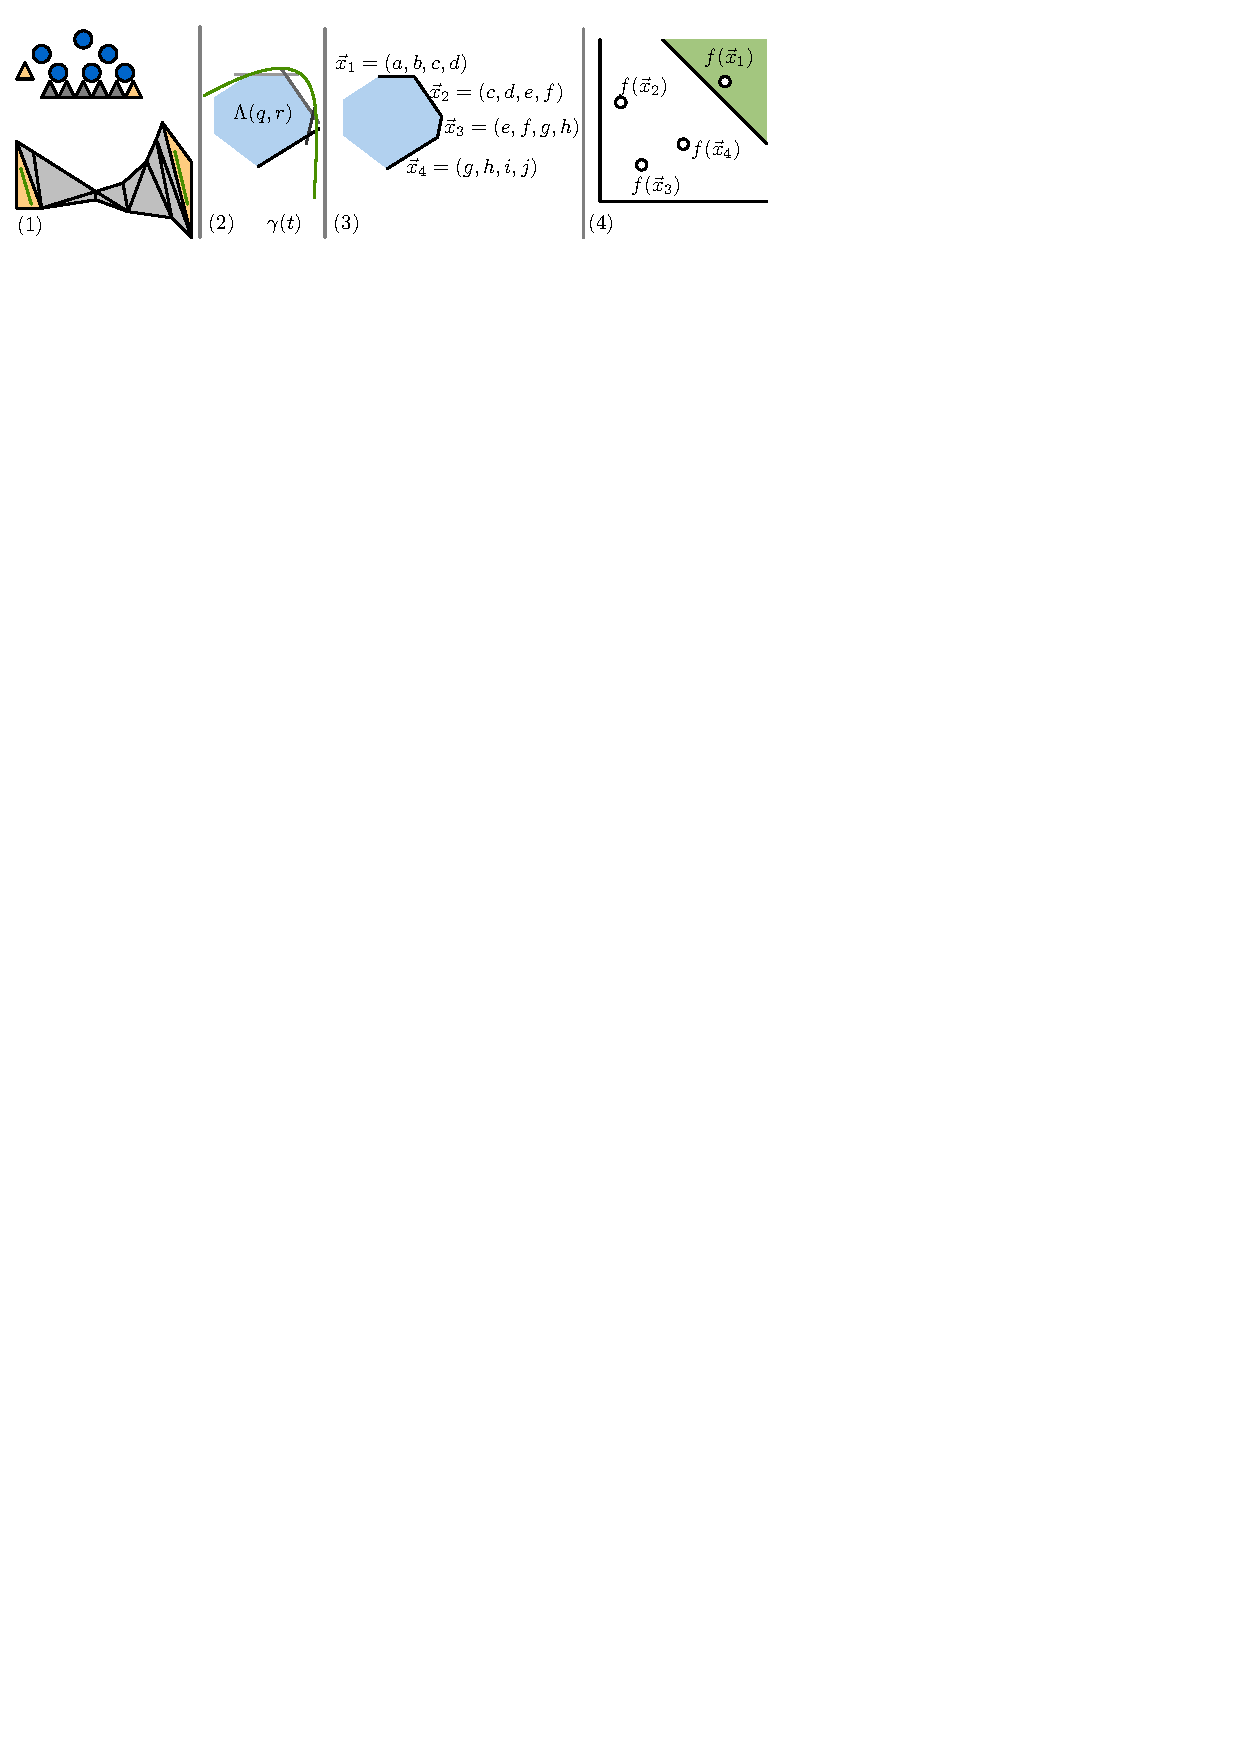
\includegraphics[]{../panel}
    \caption{(1) The base level of our data structure is a hierarchical triangulation. (2) Given $q$ and $r$, we compute the dualized visibility glass and the degree-2 query curve $\gamma$. (3) We store the parameters of each edge. (4) Each parameter vector gets mapped to a point in $\mathbb{R}^4$ and the query curve segment gets mapped to a 4-dimensional halfspace which is empty only if $\gamma$ intersects no edge from the dualized visibility glass.}
    \label{fig:panel}
\end{figure}

Our final data structure (Figure~\ref{fig:panel}) consists of two levels. The first level is a slight
variation of the two-point shortest-path query data structure of Guibas and
Hershberger~\cite{guibas1989optimal}. The data structure essentially stores a
collection of hourglasses explicitly (unlike in the original data structure). For each pre-stored hourglass, its boundary vertices are in leaves of a binary search tree and internal nodes of these trees correspond to subchains. Each internal node $v$ corresponds to a subchain $C_v$ and stores an associated data structure $\Delta_v$. We dualize the
supporting-lines of the edges in $C_v$ to points. This essentially dualizes $C_v$ into another polygonal chain in the dual. The associated structure $\Delta_v$ stores not only the  edges of this dual chain, but also for each edge a specific point in $\mathbb{R}^k$. This allows $\Delta_v$ to answer the intersection query using halfspace emptyness queries.

 When we get a query consisting of the line-segments $e_1, e_2$
representing the trajectories of $q$ and $r$, we have to decide if there exists
a time $t^*$ at which $q$ and $r$ can see each other. The main idea is to query
our data structure for the visibility-glass $L(e_1, e_2)$ and we obtain $L(e_1, e_2)$ as a collection of $\mathcal{O}(\log^2 n)$ nodes. These nodes together store the dual visibility glass $\Lambda(e_1, e_2)$. Given $e_1, e_2$, we can compute the dual query hyperbola $\gamma(t)$ and its degrees of freedom $\vec{a}$ in constant time. We then for each node $v$, query its associate data structure $\Delta_v$ to detect an intersection between $\gamma(t)$ and a part of $\Lambda(e_1, e_2)$. It follows from our formulation of the predicate function (which specifies if there is an intersection between $\gamma(t)$ and $\Lambda(e_1, e_2)$) that the total query time is $O(n^{1 - \frac{1}{16000} + \varepsilon})$.
%
%\begin{co

\bibliographystyle {abbrv}
\bibliography {bib}

\appendix


\begin{comment}
\section* {Appendix}
To supplement the abstract on the previous two pages, 
we now provide a complete full version of our paper.

\section {Introduction}

\subparagraph {Trajectories.}
A \emph {trajectory} is a 
sequence of time-stamped locations 
in the plane, or more generally in $\R^d$, which
models the movement of an entity.
Trajectory data is obtained by tracking the movements of e.g. animals \cite{BovetB88,Calenge200934,gal-nmibc-09}, hurricanes \cite{Stohl1998947}, traffic \cite{lltx-dftf-10}, or other moving entities \cite{dwf-rpm-09} over time.
Large amounts of such data have recently been collected in a variety of research fields.
As a result, there is a great demand for tools and
techniques to analyze trajectory data, and many innovative algorithmic solutions have been recently developed in computational geometry~\cite{bbgll-dcpcs-11,grsc-pcecu-07,gs-tcmrm-99,lhw-tc-07,vgk-dsmt-02}.
%\maarten {Cite a survey.}

\subparagraph {Visibility.}

\emph{Visibility} is one of the most studied topics in computational geometry~\cite {moet,welzl1985constructing,POCCHIOLA1996279}.
Many different terms, like art-gallery problems, guarding, or visibility itself, have been used during the last three decades to refer to problems related to the question of whether two object are \emph{visible} from each other, amidst a number of obstacles.
and even more in adjacent fields such as computer graphics~\cite {Durand00amultidisciplinary}, Geographic Information Science (GIS)~\cite{FM03}, and robotics~\cite {moet}, to name just a few.
Within computational geometry, Gosh and Giswani compiled a survey of {\em unsolved} problems in this area~\cite {Ghosh:2013:UPV:2543581.2543589}.
Buchin~\etal recently studied visibility between {\em uncertain} points~\cite {bkls-rbavil-19}, and as a subroutine solve the question of whether two points can see each other (improving an earlier result by Rote~\cite{r-dc-13} from $O(n^9)$ time to $O(n^2)$).

\subparagraph {Trajectory visibility.}

A natural question to ask, with numerous applications, is whether two entities following different trajectories in a scene with obstacles that block visibility, can see each other.
Somewhat surprisingly, given the amount of research in both trajectories and visibility, almost no previous work in this direction exists.
Part of the reason may be that studying trajectories in {\em context} is still relatively new to this area, and context is essential for meaningful question.
When studying visibility between trajectories as opposed to static objects, the role of {\em time} is essential: we are not interested whether there exists visibility between two geometric shapes, but rather whether there exists a {\em time} at which two point objects are visible. This makes the question fundamentally different from existing work in visibility.

\subparagraph {Data structures.}

In many analysis applications, trajectories live in a static environment (the obstacles), but new trajectories arise over time. This raises the natural question whether one can store the environment in a data structure that can support visibility queries between trajectories.
%\maarten {In a later version, we should work out some of these applications. One of them is sampling from a distribution (our original one), but I'm sure there are many other scenarios in which the environment doesn't change, but the trajectories do. :)}
Solutions for the same question for point-to-point visibility are well-known.
Guibas and Hersberger \cite{guibas1989optimal} present a linear-size data structure on a simple polgyon which can return the shortest path between a pair of query points in logarithmic time. Note that the points are mutually visible if and only if their shortest path is a single line segment.
%\maarten {Find out about earlier solutions for this problem.}

\subparagraph {Trajectory planning.}

In contrast to {\em testing} visibility between trajectories, there is a considerable body of previous work on trajectory {\em planning} under visibility contraints (points should remain mutually visible) or with the aim to maximize visibility.
Shkurti and Dudek~\cite {6907405} consider the complementary problem: how can we plan the trajectories of two moving objects to maximize visibility between them.
This problem is also closely related to {\em camera planning}~\cite {christie}, where one trajectory is given as input but a second one should be chosen to maintain visibility between the two points.
%\maarten {Eventually we should do a more thorough review of this area.}


\subparagraph {Formal problem statement.}

  Given a simple polygon $P$, preprocess $P$ into a data structure that can answer queries of the following type: given two trajectories $T_1$ and $T_2$ that represent the motion of two moving entities $q(t)$ and $r(t)$ within $P$, is there a time $t^*$ such that the segment $\overline{q(t^*)r(t^*)}$ is contained in the interior of $P$?

\subparagraph {Our results.}

  If we denote by $n$ the complexity of $P$, and by $\tau$ the total complexity of the two query trajectories, we obtain the following result:
  We can preprocess $P$ in 
  polynomial $\mathcal{O}(n^{1+\varepsilon})$
  time into a data structure using 
  polynomial $\mathcal{O}(n^{1+\varepsilon}$
  space, such that a query can be answered in 
  time which is linear in $\tau$, but sublinear in $n$.
  
  In the following, we restrict our attention to the case where $T_1$ and $T_2$ are single line segments, since more complex queries can be reduced to this case by simply querying each pair of contemporary segments (if the vertices of $T_1$ and $T_2$ are not time-aligned, we insert $O(\tau)$ additional vertices to make this be the case).





\section{Hourglasses}


\begin{figure}[h]
    \centering
    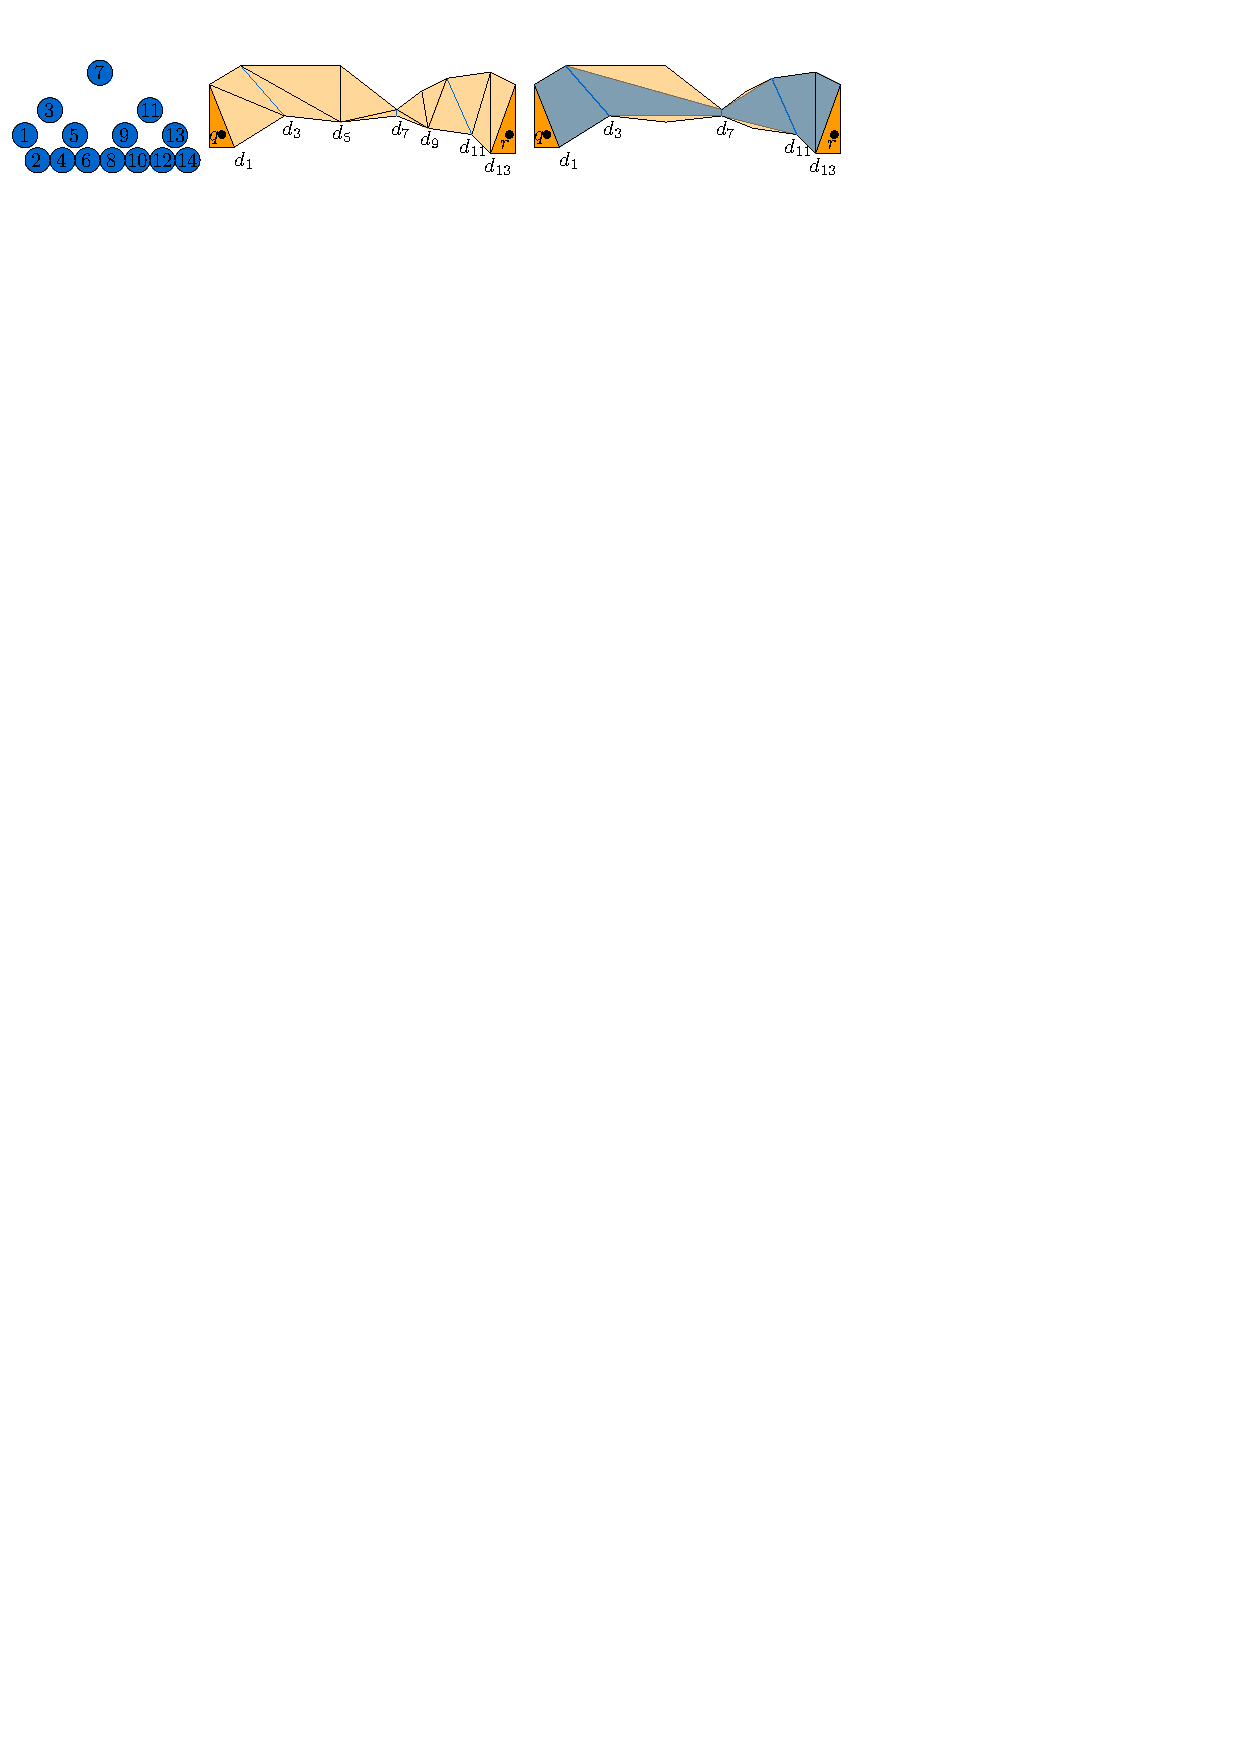
\includegraphics[]{../guibas}
    \caption{A triangulated polygon $P$ where the diagonals are labelled from $d_1$ to $d_14$. Left we see a balanced hierarchical subdivision on the diagonals. Suppose we want to know the shortest path between $q$ and $r$. Then there are $13$ diagonals (and thus $13$ triangles) between $q$ and $r$. However, the Guibas and Hershberger data structure has pre-stored the hourglasses $H(d_1,d3)$, $H(d_3, d_7)$, $H(d_7, d_11)$ and $H(d_{11}, d_{13})$. Thus during query time, we only have to concatenate $\log n$ hourglasses. }
    \label{fig:guibas}
\end{figure}

Guibas and Hershberger \cite{GuibasHS91} studied shortest path queries within a simple polygon $P$. In their paper they define the concept of an \emph{hourglass}: for any two line segments $\ell_1, \ell_2$ in $P$, the \emph{hourglass} $H(\ell_1, \ell_2)$ is the union of all shortest paths from any point on $\ell_1$ to any point on $\ell_2$. They show that the hourglass is a polygon within $P$ (where the polygon could have a passage of width 0), bounded by the shortest paths between the endpoints of $\ell_1, \ell_2$ together with $\ell_1, \ell_2$ itself. It could be that the first endpoint of $\ell_2$ is contained within the polygon spanned by $\ell_1$ and the shortest paths between $\ell_1$ and the second endpoint of $\ell_2$. This special case realises a \emph{funnel} and it is easy to check visibility in a funnel. Since the hourglass is bounded by a collection of paths in $P$, the hourglass can be represented as a binary search tree where each node in the tree represents a vertex in a shortest path bounding $H(\ell_1, \ell_2)$. Guibas and Hershberger call this representation the \emph{implicit representation} \cite{guibas1989optimal}.

Guibas and Hershberger build a balanced hierarchical subdivision of $P$ using its diagonals~\cite{guibas1989optimal}. A balanced hierarchical subdivision is essentially a balanced binary tree in which every node corresponds to a subpolygon of $P$ and a diagonal that splits the subpolygon into two smaller subpolygons (refer to Figure~\ref{fig:guibas}). The subpolygon of the root is $P$ itself. The subpolygons of the leaves of the tree form a triangulation of $P$. 
Additionally, each node in the binary tree stores the implicit representation of the hourglasses between the diagonals on this subpolygon. A shortest path query between any two points $q,r \in P$ is answered in four steps: first they locate the two leaf cells in our binary tree whose triangles contain $q$ and $r$. Second they identify the sequence of $m$ diagonals $d_1, d_2, \ldots, d_m$ of $P$ that lie in between these two triangles (there could be linearly many diagonals). 
Guibas and Hershberger show that the hourglass between $d_1$ and $d_m$ consists of at most $\mathcal{O}(\log n)$ pre-stored hourglasses of $P$ and as a third step, they concatenate these at most $\mathcal{O}(\log n)$ hourglasses into the hourglass $H(d_1, d_m)$. Lastly, they compute the shortest path between $q$ and $d_1$ and $r$ and $d_m$ using $H(d_1, d_m)$. 

Suppose that for a time $t^* \in [0,1]$, the points $q(t^*)$ and $r(t^*)$ can see one another. Then the visibility line between $q(t^*)$ and $r(t^*)$ is also the shortest path between $q(t^*)$ and $r(t^*)$. We use the Guibas and Hershberger data structure to compute the shortest paths between all endpoints of $e_1$ and $e_2$ to compute the hourglass $H(e_1, e_2)$. If there is a time $t^* \in [0,1]$ such that the points can see one another, then we know that their line-of-sight is contained within $H(e_1,e_2)$.

\subparagraph*{Visibility glass.}

Above we mentioned that if $q$ and $r$ can see one another, then their line-of-sight is contained within the hourglass $H(e_1, e_2)$. The line-of-sight between the points is always a line segment, but $H(e_1, e_2)$ contains many more shortest paths. For any two line segments $\ell_1, \ell_2$, we define the \emph{visibility glass} denoted by $L(\ell_1, \ell_2)$ as the collection of \emph{line segments} from points on $\ell_1$ to points on $\ell_2$ that are contained in $P$. 
Observe that the visibility glass may be the empty set, and the segments of the visibility glass between $\ell_1$ and $\ell_2$ are always a subset of the hourglass of $\ell_1$ and $\ell_2$. See Figure \ref{fig:visibilityglass} for an illustration. We can obtain the visibility glass, by querying the Guibas and Hershberger data structure twice using the following observation from Chazelle \cite{Chazelle1989} (Lemma 2.1):

\begin{observation}
For any two line segments $\ell_1, \ell_2 \in P$, there exist two line segments $\ell_1' \subset \ell_1, \ell_2' \subset \ell_2$ such that $L(\ell_1, \ell_2) = H(\ell_1', \ell_2')$. Moreover, $\ell_1'$ and $\ell_2'$ are given by the bitangents of $H(\ell_1, \ell_2)$.
\end{observation}


Suppose that for two segments $e_1, e_2$ the visibility glass is not a funnel. Then the visibility glass is the hourglass of two line segment $e_1', e_2'$. The hourglass $H(e_1, e_2)$ is bounded by $e_1$, $e_2$ and two semi-convex subchains which we will call the upper and lower chain. Denote with $\pi_1$ the shortest path from the left-most point of the upper chain to the right-most point of the lower chain, and denote with $\pi_2$ the shortest path between the other two remaining endpoints of $e_1'$ and $e_2'$. The paths $\pi_1$ and $\pi_2$ both partially coincide with the upper and lower chain, and their coinciding parts are connected by a single line segment whose extension forms a bitangent. Using the data structure of Guibas and Hershberger, we can obtain the paths $\pi_1$ and $\pi_2$ in their implicit representation (that is, a forest of nodes). Note that both bitangent edges are the only edges on $\pi_1$ and $\pi_2$ which start with a clockwise rotation and end with a counter-clockwise rotation. We binary search the two forests returned by Guibas and Hershberger for these two bitantents. Given the two bitangents, we identify $e_1'$ and $e_2'$ and we re-use the data structure to obtain the implicit representation of the visibility glass $L(e_1, e_2)$.

\begin{figure}[tb]
    \centering
    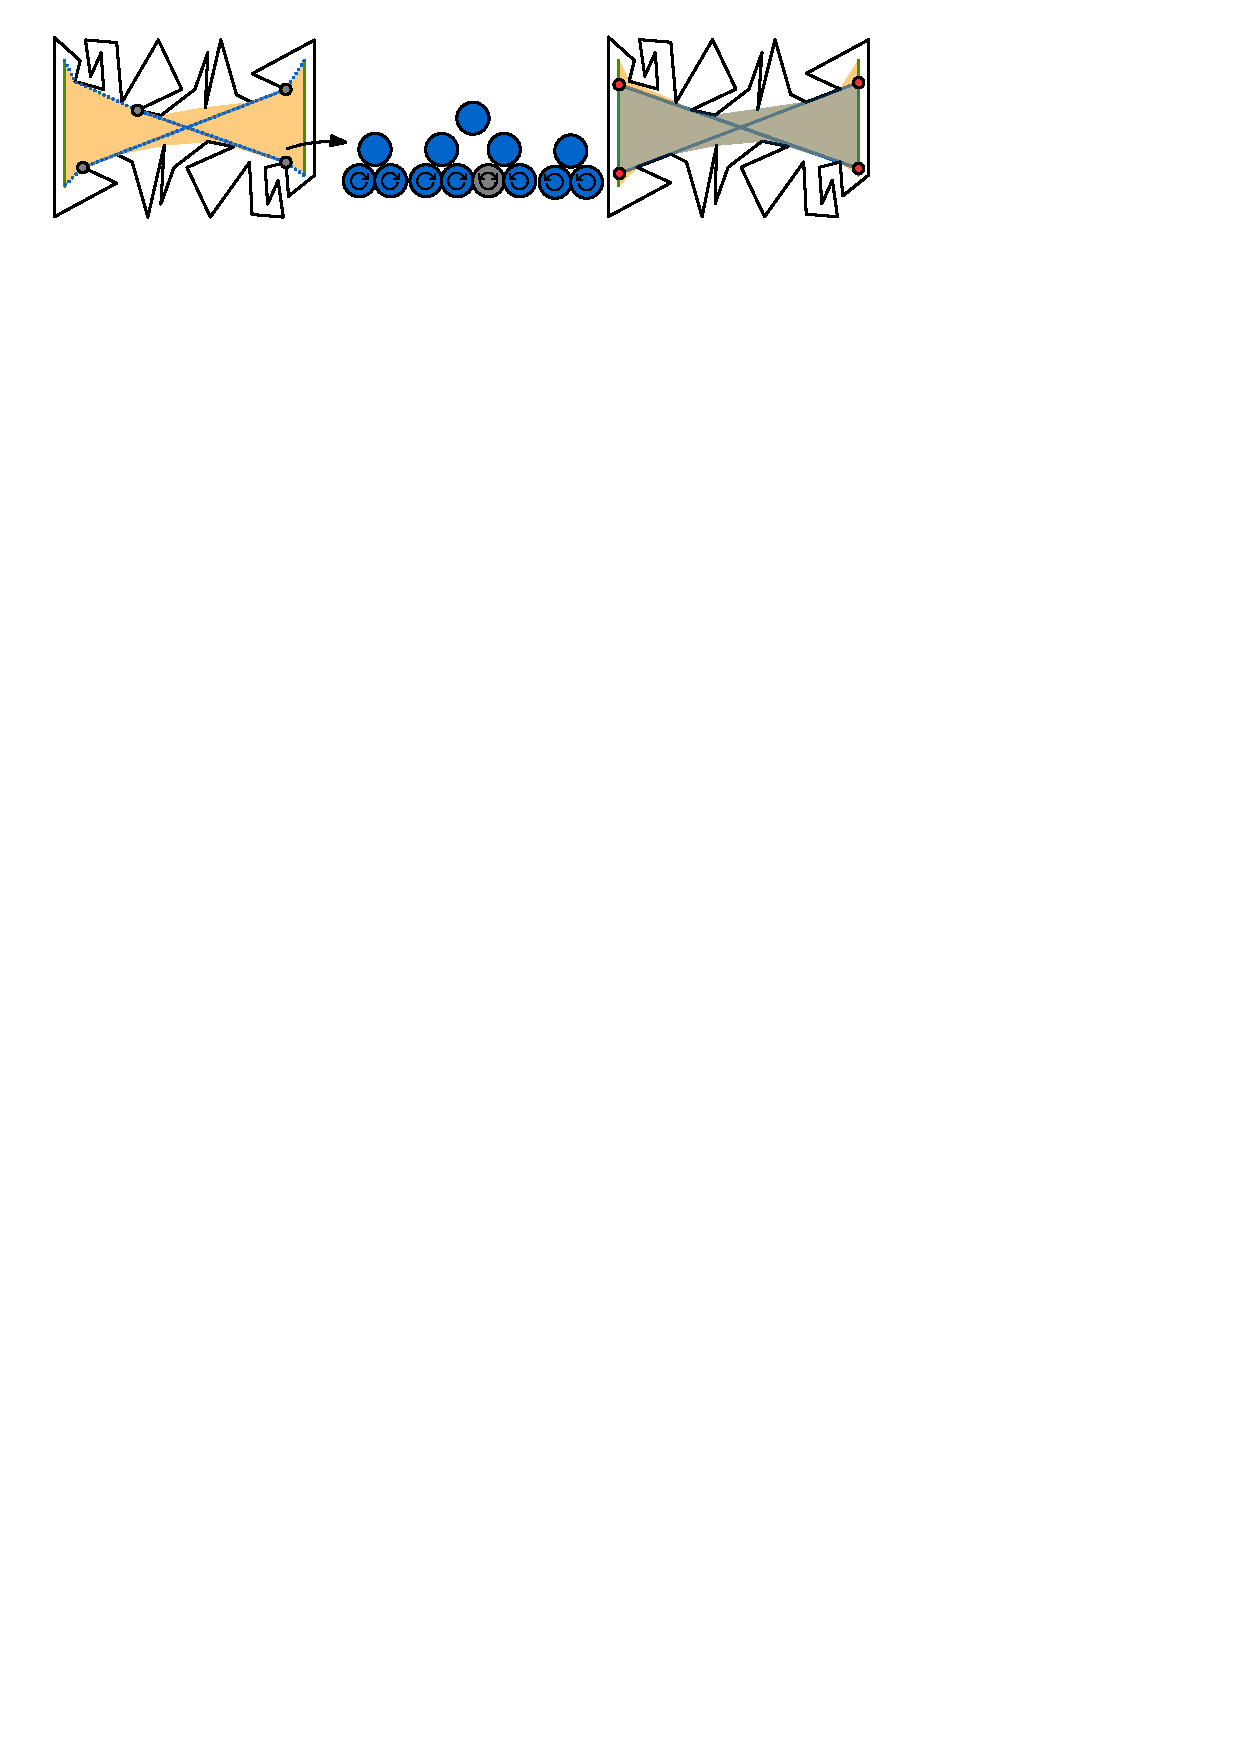
\includegraphics[]{../visibilityglass}
    \caption{The two trajectories $e_1$ and $e_2$, one from $q(0)$ to $q(1)$ and the other from $r(0)$ to $r(1)$. $H(e_1, e_2)$ is blue + orange, $L(e_1, e_2)$ is blue. Note that $e_1'$ ends in a bitangent in grey that is supported by an edge on the shortest path from $q(1)$ to $r(1)$.}
    \label{fig:visibilityglass}
\end{figure}




\section{Visibility as an intersection}


At time $t \in [0,1]$, the line segment $\overline{q(t)r(t)}$ is the line-of-sight between the two points. The points can see one another at time $t$ if and only if the segment $\overline{q(t)r(t)}$  is contained within the visibility glass $L(e_1, e_2)$. Therefore we can answer our query by checking if there is a time $t^*$ such that $\overline{q(t^*)r(t^*)}$ is contained in $L(e_1,e_2)$ (and therefore in $P$). We check this as follows:
it is known \cite{Chazelle1989} that the dual of the visibility glass is a
convex polygon with at most $n$ edges and we denote this polygon by
$\Lambda(e_1,e_2)$. For all $t \in [0,1]$, we denote the dual of the line
$q(t)r(t)$ by the point $(\alpha(t), \beta(t))$, this point traces out a curve
$\gamma(t)$ (Equation~\ref{eq:curve}). A point of the query curve $\gamma(t)$
is contained in $\Lambda(e_1,e_2)$ only if: either $\gamma(t)$ is contained in,
or intersects the boundary of $\Lambda(q,r)$.
If $\gamma(t)$ is contained in $\Lambda(e_1, e_2)$, the entities can always see one another and since this is easy to verify we assume that this is not the case. Thus we only need to check if there is a time $t^*$ such that $\gamma(t)$ intersects the border of $\Lambda(e_1, e_2)$. We answer this intersection query with the linarization techniques from Agarwal \etal \cite{agarwal2013range}. 


For ease of notation, we assume that the entity $q$ walks from $(a_1, a_2)$ to $(a_1 + a_3, a_2 + a_4)$ and that the entity $r$ walks from $(a_5, a_6)$ to $(a_5 + a_7, a_6 + a_8)$, both during the time interval $[0,1]$. Now we can parametrize the position of entity $q$ and $r$ as follows:

\begin{equation}
    \label{eq:line}
     q(t) = \left( \begin{array}{c}
         x_{q(t)}  \\
         y_{q(t)} 
    \end{array}  \right) = 
    \left( \begin{array}{c}
         a_1 + a_3 t \\
         a_2 + a_4 t
    \end{array}  \right)  \quad
      r(t) = \left( \begin{array}{c}
         x_{r(t)}  \\
         y_{r(t)} 
    \end{array}  \right) = 
    \left( \begin{array}{c}
         a_5 + a_7 t \\
         a_6 + a_8 t
    \end{array}  \right) 
\end{equation}


At all times, the line $\gamma(t)$ represents the line through $q(t)$ and $r(t)$. We say that at all times, $\gamma(t)$ has slope and offset $(\alpha, \beta)$. The parametrisation of $\gamma(t)$ then becomes:

\begin{equation}
\label{eq:curve}
   \gamma(t) = \left( \begin{array}{c}
         \alpha(t)  \\
         \beta(t) 
    \end{array}  \right) = 
    \left( \begin{array}{c}
         \frac{y_{r(t)} - y_{q(t)}}{x_{r(t)} - x_{q(t)}}  \\
         \alpha(t)\cdot x_{q(t)} - y_{q(t)}
    \end{array}  \right) =
    \left( \begin{array}{c}
         \frac{ a_6 - a_2 + (a_8 - a_4) t}
      { a_5 - a_1  + (a_7 - a_3) t }  \\
         \alpha(t) (a_1 - a_3 t) - a_2 - a_4 t 
    \end{array}  \right)
  \end{equation}
  
  If the time $t$ lies between $0$ and $1$, this parametric equation traces our hyperbolic segment. If we take $t$ over all of $\mathbb{R}$, the parametric equation traces a full hyperbola. For reasons that will become apparent later, we opt to rewrite the hyperbolic curve to a canonical form that drops the dependence on $t$. First we take the formula for the $\beta$-coordinate and isolate $t$:
  
  \[
     t = \frac{\alpha(t) a_1 - a_2  - \beta(t)}{\alpha(t) a_3 + a_4}
  \]
We then take the formula for the $\alpha$-coordinate and remove the fraction by multiplying both sides with $ ((a_5 - a_1)  + (a_7 - a_3) t)$:

\[ 
\alpha(t)(a_5 - a_1)  + \alpha(t)(a_7 - a_3) t = (a_6 - a_2) + (a_8 - a_4) t
\]

We substitute the value for $t$ into this equation, and remove the fraction by multiplying both sides with $(\alpha(t) a_3 + a_4)$:

\begin{align*}
\alpha(t)(\alpha(t) a_3 + a_4)(a_5 - a_1)  + \alpha(t)(a_7 - a_3) (\alpha(t) a_1 - a_2  - \beta(t)) = \\
(a_6 - a_2)(\alpha(t) a_3 + a_4) + (a_8 - a_4) (\alpha(t) a_1 - a_2  - \beta(t)) \Rightarrow \\
\alpha(t)^2a_3(a_5 - a_1) + \alpha(t)a_4(a_5 - a_1)  + \alpha(t)^2a_1(a_7 - a_3)
- \alpha(t)a_2(a_7 - a_3)  - \alpha(t)\beta(t)(a_7 - a_3) = \\
\alpha(t) a_3(a_6 - a_2) + a_4(a_6 - a_2) + \alpha(t)a_1(a_8 - a_4) - a_2 (a_8 - a_4) - \beta(t)(a_8 - a_4) 
\end{align*}

Lastly, we take all variables to one side and we group on terms based on $\alpha$ and $\beta$ and we remove redundancies

\begin{align*}
    0= [\alpha(t)^2](a_5 a_3 -2 a_1 a_3 + a_1 a_7)+ \\
    [\alpha(t)](a_4 a_5 - a_3 a_6 + a_2 (2 a_3 - a_7) - a_1 a_8) + \\
    [\alpha(t)\beta(t)](-(a_7 - a_3)) + [\beta(t)](-(a_8 - a_4)) + [1](a_4(a_6 - a_2)- a_2 (a_8 - a_4))
\end{align*}

\section{Detecting an intersection between a hyperbolic segment and a convex polygon.}

Suppose we are given a set $E$ of $n$ edges which form a convex polygon $P_E$. In this section we show how to preprocess $E$ such that for any hyperbolic segment $\gamma$, we can test whether $\gamma$ intersects the polygon or not in sub-linear time. We assume that we are given $\gamma$ as an equation of the form:


\begin{figure}[h]
    \centering
    \includegraphics[]{../intersection}
    \caption{ If the hyperbolic segment $\gamma$ intersects $P_E$, then either (a) at least one endpoint of $\gamma$ lies within the polygon, (b) the hyperbolic segment cuts off a vertex and $\gamma(t)$ intersects an edge connected to that vertex (c) the hyperbolic segment intersects only one edge of $E$ twice.}
    \label{fig:intersection}
\end{figure}

\begin{equation}
    \label{eq:hyperbola}
    0 = A_1 x_1^2 + A_2 x_1 + A_3 x_1x_2 + A_4 x_2 + A_5 x_2^2 + A_6, \quad (a_1, a_2), (a_3, a_4) \in \mathbb{R}^2
\end{equation}

Where $A_1, A_2 \ldots A_6$ are arbitrary constants that determine the shape of the full hyperbola, $(x_1, y_1)$ is the start coordinate of the hyperbolic segment $\gamma$ and $(x_2, y_2)$ are its end coordinates. Note that for any other representation of the hyperbolic segment, we can compute these values in constant time. Observe that if the hyperbolic segment $\gamma$ intersects the polygon formed by $E$, then there can be three cases of intersection, denoted by $(a), (b), (c)$ and illustrated by Figure~\ref{fig:intersection}:



We detect an intersection of case $(a)$ and $(c)$ using a hierarchical triangulation of $P_E$: given $P_E$ we find a vertex $v_{r0}$ of $P_E$ and an edge $(v_{r1}, v_{r2}) \in E$ such that the triangle $T_r$ formed by $v_{r0},v_{r1}, v_{r2}$ separates $P_E$ into two convex polygons of roughly equal size. The separating triangle $T_r$ becomes the root of the hierarchical decomposition and we recurse.


\paragraph*{Solving case (a).}
Suppose we are given an endpoint $g$ of the hyperbolic segment $\gamma$ and we want to know if the endpoint lies within $P_E$ (refer to Figure~\ref{fig:triangulation} (a)). We traverse the hierarchical triangulation of $P_E$ as follows: we check if $g$ lies within $T_r$: the triangle at the root of the hierarchical decomposition. If it does, the endpoint must lie within $P_E$. The edges $(v_{r0}, v_{r1})$ and $(v_{r0}, v_{r2})$ coincide with the two sub-polygons of $P_E$ and $w.l.o.g$ we say that $(v_{r0}, v_{r1})$  lies to the left and $(v_{r0}, v_{r2})$ lies to the right. We look at the halfline from $v_{r0}$ through $v_{r1}$ and we form a quantile by taking a perpendicular vector to the left. The left sub-polygon is contained in this quantile and $g$ could therefore only be contained in the left sub-polygon if it is contained in this quantile. A symetric property holds for the right sub-polygon. We identify wheter $g$ could lie in the left or right sub-polygon in constant time and we recurse.


\begin{figure}[h]
    \centering
    \includegraphics[]{../triangulation}
    \caption{ (a) The three vertices $v_{r0}, v_{r1}, v_{r2}$ that form the triangle $T_r$ and the left quantile. (b) The three vertices $v_{r0}, v_{r1}, v_{r2}$ that form the triangle $T_r$ and the two supporting lines of $(v_{r0}, v_{r1})$ and $(v_{r0}, v_{r2})$}
    \label{fig:triangulation}
\end{figure}



\paragraph*{Solving case (b).}
Suppose we are given a hyperbola $\gamma$ and we want to find the unique segment that is stabbed twice by $\gamma$ (if any exists) (refer to Figure~\ref{fig:triangulation} (b)). We traverse the hierarchical decomposition of $P_E$ as follows: we check if $\gamma$ intersects any edge of the root triangle $T_r$. If $\gamma$ intersects such an edge edge, then we have found an intersection between $\gamma$ and $P_E$. If not then w.l.o.g we assume that the two remaining sub-polygons of $T_r$ lie to the left and to the right. Now imagine the segment $(v_{r0}, v_{r1})$. This segment is intersected by two edges of the left sub-polygon of $E$. If we take the edge $(v_{r0}, v_{r1})$ and two halflines through these segments, we cut off a space to the left which is the union of three halfplanes (Figure~\ref{fig:triangulation}). The query curve $\gamma$, can only intersect a unique edge in the left sub-polygon twice if it is contained within this left space. A similar property holds for the edge $(v_{r0}, v_{r2})$ and its induced right space. If $\gamma$ is contained within both spaces, $\gamma$ can never intersect $P_E$. These observations allow us to identify the unique sub-polygon of $P_E$ that could be intersected by $\gamma$ and we recurse. 


\paragraph*{Solving case $(c)$.}

Consider the full hyperbola $\gamma$, it partitions the plane into two spaces which we shall call the interior and the exterior. An edge $(v_1, v_2)$ is intersected by $\gamma$ only once, if $v_1$ lies in the interior and $v_2$ lies in the exterior or vice versa. So to find an edge that is intersected by the full hyperbola $\gamma$, we only have to find a pair of adjacent vertices with this property. However, in this problem, we are given a hyperbolic segment and not a full hyperbola. There could be linearly many edges in $P_E$ which are intersected by the full hyperbola $\gamma$, and only one edge which is intersected by the hyperbolic segment $\gamma(t)$. However, let $E' = (e_1, e_2, e_3 \ldots e_m)$ be $m$ edges in clockwise order, which are intersected by an arbitrary hyperbola $\gamma$. Let $\gamma(t)$ be any segment of the hyperbola $\gamma$ and let $\gamma(t)$ intersect $k$ edges of $E'$. Then these $k$ edges must be consecutive edges in the clockwise order. Our approach to find an edge which is intersected by $\gamma(t)$ is as follows: we first obtain the $m$ edges $E'$ which are intersected by the full hyperbola $\gamma$ in some treelike representation using semi-algebraic range searching. We then perform binary search on $E'$ to find the consecutive edges of $E'$ that are intersected by the query segment (if any) in logarithmic time.

\paragraph*{Semi-algebraic range searching.}


Let $S$ be a set of $n$ points in $\mathbb{R}^d$ for a constant dimension $d$. Let $\Gamma$ be a family of geometric regions (called semi-algebraic ranges) in $\mathbb{R}^d$ where each region $G \in \Gamma$ is bound by an algebraic curve $\gamma$ which is parametrised by a vector $\vec{a} = (a_1, a_2 \ldots a_m)$ for some integer $m$. Imagine we are interested in preprocessing $S$, such that for any range $\Gamma$, we can specify which points of $S$ lie within this range. This problem was studied (in a more general form) by Agarwal \etal in \cite{agarwal2013range} and there they obtain the following result:

Suppose that you can derive a predicate function $F(\vec{x}, \vec{a}) \le 0$ that for any point $\vec{x}$ and any range $\Gamma$ parametrised by a vector $\vec{a}$, specifies if $\vec{x}$ lies within $\Gamma$. Moreover, this function is of the form: $F(\vec{x}, \vec{a}) =  g_0(\vec{a}) + \sum_{i=1}^k g_i(\vec{a})f_i(\vec{x})$ where $f_i$ and $g_i$ are polynomials dependent on $\vec{x}$ and $\vec{a}$ respectively. Then we can transform this $d$-dimensional semi-algebraic range searching problem into a halfspace range searching problem into $\mathbb{R}^k$. Specifically, Agarwal \etal prove that you can map any $d$-dimensional point $\vec{x}$ to the $k$-dimensional point $f(\vec{x}) = (f_1(\vec{x}), f_2(\vec{x}), \dots f_k(\vec{x}))$, and any query range to the $k$-dimensional halfspace $G(\vec{a}) = \left\{ \vec{y} \in \mathbb{R}^k \mid g_0(\vec{a})  + \sum_i^k g_i(\vec{a})y_i  \le C \right\}$ and that $\vec{x}$ is contained in $\Gamma$ if and only if $f(\vec{x})$ is contained in $G(\vec{a})$.  Refer to Figure~\ref{fig:algebraic} for an example. In our case, we have a hyperbola parametrised by Equation~\ref{eq:hyperbola} and points lie on the interior if and only if the righthand side of the equation is larger than the lefthand side. This immediately gives us a predicate $F(\vec{x}, \vec{A}) =  A_6 + A_1 x_1^2 + A_2 x_1 + A_3 x_1x_2 + A_4 x_2 + A_5 x_2^2 \le 0$ and if we want to equate this predicate formulation to the formulation from Agarwal \etal then $(g_0, g_1, g_2, g_3, g_4, g_5)(\vec{A}) = (A_6, A_1, A_2, A_3, A_4, A_5)$ and $(f_1, f_2, f_3, f_4, f_5)(\vec{x}) = (x_1^2, x_1, x_1x_2, x_2, x_2^2)$. It follows that we can transform our full hyperbola interior-exterior query into a $5$-dimensional halfspace range searching query. Halfspace range queries can be solved using either partition trees, cutting trees or a combination of the two, we describe a solution using partition trees.

\begin{figure}
    \centering
    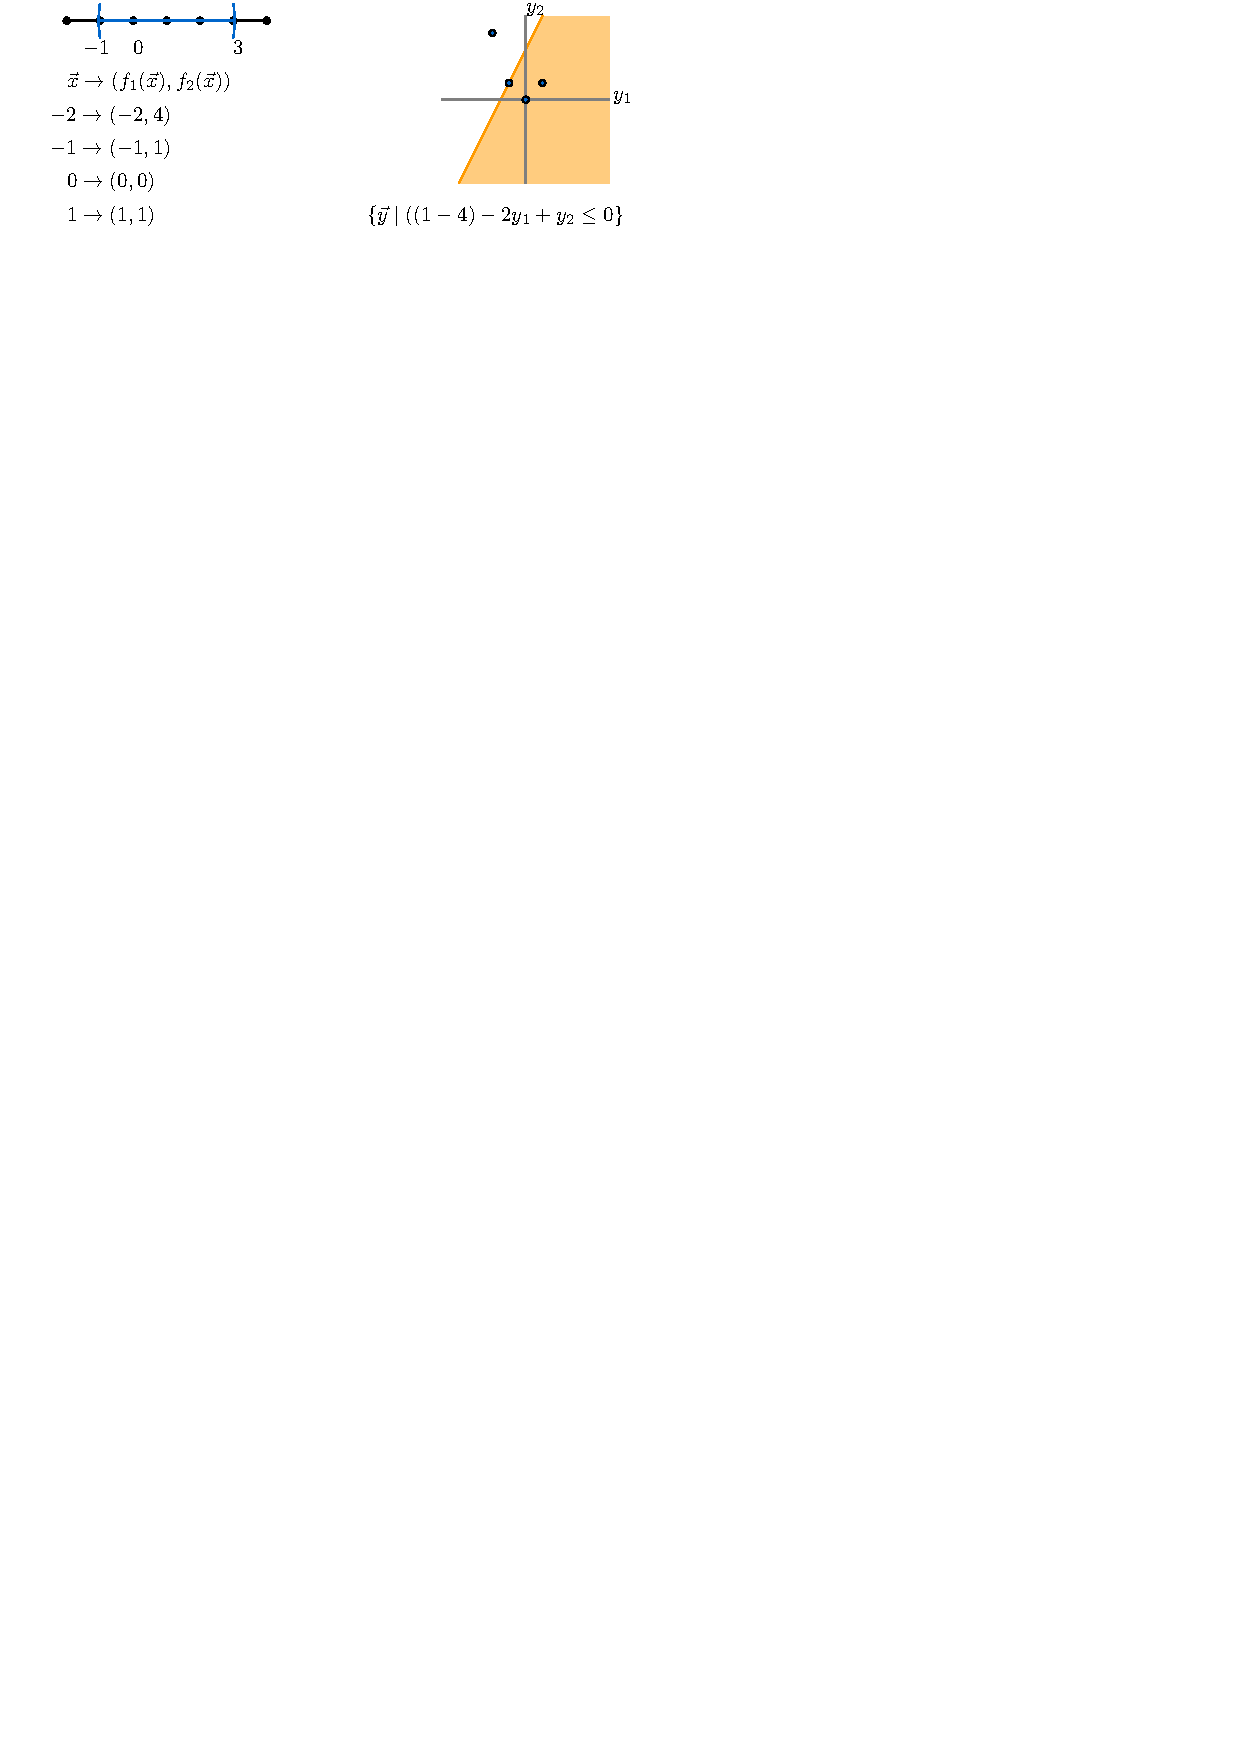
\includegraphics[]{../algebraic}
    \caption{Suppose we have a set of $n$ points in $\mathbb{R}^1$ and that our queries are the family of 1-dimensional disks with center $a_1$ and radius $a_2$. An arbitrary point parametrized by $\vec{x} = (x_1)$ intersects the disk parametrized by $\vec{a} = (a_1, a_2)$ only if $(a_1 - x_1)^2 \le a_2^2$. Hence this gives a predicate: $F(\vec{x}, \vec{y}) = (a_1^2 - a_2^2) + (-2a_1)[x_1] + (1)[x_1^2] \le 0$ which leads to a 2-dimensional halfspace emptyness query. Each query point $x_1$ gets mapped to $( f_1(x_1), f_2(x_1) ) = (x_1, x_1^2)$ and each query parametrized by $\vec{a}$ gets mapped to the halfspace: $\{ y \in \mathbb{R}^2 \mid (a_1^2 - a_2^2) - 2a_1 y_1 + 1 y_2 \le 0$. }
    \label{fig:algebraic}
\end{figure}

Knowing this, we show how to find an intersection of case $(c)$ using two copies of a three-level data structure. Let $P$ and $Q$ be the set of start and end coordinates of the edges in $E$. We only describe the first copy, the second copy is identical but has the start points lie on the exterior of the hyperbola $\gamma$ as opposed to the interior:

The first level of our data structure assigns to each two-dimensional point in $P$ a point in $\mathbb{R}^5$ according to the predicate and we store them in a 5-dimensional partition tree. Each node in the partition tree, represent a set of points $P$ whose transformation lie within a $k$-dimensional halfspace. For each node, for each of these start points of $P$, we identify their correspond endpoints in $Q$, transform them to points in $\mathbb{R}^5$ and we maintain a partition tree on top of these points. Each node in this second level partition tree, represents a set of edges of $E$ whose start points lie on the interior and end points lie on the exterior of a full hyperbola $\gamma$. We build a binary search tree on this set of edges which orders the edges clockwise. 



\paragraph*{Solving a hyperbolic intersection query.}

Given the set of edges $E$, we build a hierarchical triangulation of the polygon $P_E$ and the three-level intersection data structure described above. Given a query segment $\gamma(t)$, we identify if we have an intersection of type $(a)$ or $(b)$ in logarithmic time. If not, we query our three level data structure as described above: multi-level, five dimensional partition trees take $\mathcal{O}(n^{1 + \varepsilon}$ storage and construction time and have $\mathcal{O}(n^{\frac{4}{5} + \varepsilon}$ query time where $\varepsilon$ is an arbitrarily small positive constant. The cutting tree alternative uses $\mathcal{O}(n^5)$ storage and construction time and achieves $\mathcal{O}(\log^5 n)$ query time. The additional binary search on the clockwise order takes an additional factor $\log n$ time per query.  Thus, we can conclude the following:

\begin{theorem}
We can preprocess any convex polygon $P$ with $n$ edges in $\mathcal{O}(n^{1+\varepsilon})$ time and space, such that we can determine for any hyperbolic segment $\gamma(t)$ if $P$ is intersected by $\gamma(t)$ in $\mathcal{O}(n^{\frac{4}{5} + \varepsilon})$ time.
\end{theorem}





\section{Final data structure}


Our main data structure consists of two levels. The first level is a slight
variation of the two-point shortest-path query data structure of Guibas and
Hershberger~\cite{guibas1989optimal}. The data structure essentially stores a
collection of hourglasses that can be concatenated to obtain a shortest path
between two arbitrary points $s,t \in P$. Our data structure essentially stores a collection of hourglasses explicitly (unlike in the original data structure which uses something like persistence).The vertices on the boundary of
an hourglass are stored in the leaves of a balanced binary search
tree. Internal nodes correspond to semi-convex subchains. Each internal node $v$ stores its
subchain $C_v$ in an associated data structure. Specifically, we dualize the
supporting-lines of the edges in $C_v$ to points. Two consecutive edges produce
two points, which we again connect into polygonal chains. So for every vertex
in $C_v$ the associated data structure $\Delta_v$ actually stores a line-segment;
together these segments again form a polygonal chain $\Psi_v$. The associated
data structure will support intersection queries with a hyperbolic query
segment $\gamma(t)$; i.e.~it will allow us to report the segments of $\Psi_v$
intersected by $\gamma(t)$. We implement $\Delta_v$ using the data structure from
Lemma~\ref{lem:intersection_data_structure}.

\begin{lemma}
  \label{lem:space_dual_chains}
  The total size of all chains $\Psi_v$ over all nodes $v$ is $O(n\log^3 n)$.
\end{lemma}

\begin{proof}
  The Guibas and Hershberger data structure is essentially a balanced
  hierarchical subdivision that recursively partitions the polygon into two
  roughly equal size subpolygons. Every subpolygon has $O(\log n)$
  diagonals~\cite{guibas1989optimal}, and thus stores at most $O(\log^2 n)$
  hourglasses. It follows that all hourglasses of a subpolygon of size $m$ have
  use at most $O(m\log^2 n)$ space. The height of the balanced hierarchical
  subdivision is $O(\log n)$, and at every level the total size of the
  subpolygons is $O(n)$. Therefore, the total size of all subpolygon is
  $O(n\log n)$. The lemma follows.
\end{proof}

For a chain of size $|\Psi_v|$ the data structure $\Delta_v$ has 
polynomial %$O(ZZZZZZZZ)$
size and can be built in 
polynomial %$O(YYYYY)$
time. It follows that the total space used by our data structure is
also polynomial. %$O(...)$. 
The total preprocessing time is 
polynomial. %$O(...)$.

\subparagraph{Querying} When get a query consisting of the line-segments
representing the trajectories of $r$ and $q$, we have to decide if there exists
a time $t^*$ at which $r$ and $q$ can see each other. The main idea is to query
our data structure for the visibility-glass of the line-segments making up
these trajectories. We then dualize the visibility glass $\Lambda(e_1,e_2)$ into a convex
polygon $\Lambda(e_1,e_2)$. To test if $r$ and $q$ can see each other, we then test if the
hyperbolic segment representing the trajectories of $r$ and $q$ intersects
$\Lambda(e_1,e_2)$.

We use the first level of our data structure to report the visibility-glass $L(e_1,e_2)$
of $r$ and $q$. This is visibility glass is bounded by two inward-convex chains
$\geod(r_1,q_1)$ and $\geod(r_2,q_2)$ and two line segments $\overline{r_1r_2}$
and $\overline{q_1q_2}$. Since $\geod(r_1,q_1)$ ($\geod(r_2,q_2)$) is actually
a shortest path in $P$, we can obtain it by concatenating $O(\log n)$ of the
pre-stored hourglasses. To concatenate two hourglasses we actually select two
contiguous subchains in both hourglasses, and compute two bridge edges
connecting them. Such a contiguous subchain can be represented by $O(\log n)$
nodes in the binary search trees representing the hourglass boundary. It
follows that $\geod(r_1,q_1)$ can be represented by $O(\log^2 n)$ nodes; each
representing a pre-stored subchain in the data structure, together with
$O(\log^2 n)$ line-segments (the bridge segments). We now observe that the
chains stored in the associated data structures of these nodes, again together
$O(\log^2 n)$ separate line segments $\Xi$, actually represent the dual $\Lambda(e_1,e_2)$ of
$L(e_1,e_2)$. To check if the hyperbolic query segment $\gamma$ intersects $\Lambda(e_1,e_2)$ we check if
one of the endpoints of $Q$ lies in $\Lambda(e_1,e_2)$; in this case one of the paths
$\geod(r_1,q_1)$ or $\geod(r_2,q_2)$ is actually a single segment, or if $\gamma$
intersects the boundary of $\Lambda(e_1,e_2)$. To this end, we query each of these
associated data structures. We test for intersection with the segments in $\Xi$
separately. This yields a total query time
which is sublinear. %of $O(ZZZZZ)$.
%
%\end{comment}




\section{One ghost $r$ and one dead monkey $q$}

In this setting, we have one entity $r$ that walks a straight line segment (possibly though the edges of $P$) and an entity $q$ which is stationary at a point within the simple polygon $P$.
We say that entity $r$ walks along the line $\rho := \{ x,y \mid  0 = a_1 x - a_2 - y \}$ from the point $(A_1, A_2)$ to the point $(A_3, A_4)$ in the time interval $t \in [0,1]$. Entity $q$ is stationary at the point $(a_3, a_4) \in P$ and without loss of generality we claim that $q$ lies below $\rho$. 
Aronov \etal \cite{Aronov2002} study how to find the \emph{visibility polygon} of a query point $q$ within a simple polygon. For any polygon $P$ with $n$ edges and point $q \in P$, its visibility polygon denoted by $V_q$ is the union of all the points in $P$ which are visible from $q$. $V_q$ is a polygon with at most $n$ edges. The vertices of $V_q$ either coincide with vertices of $P$, or lie on edges of $P$. We call these latter edges \emph{uncertain edges}. The vertex on an uncertain edge, is the intersection of the line through $q$ and a reflex vertex of $P$. We call for any query point $q$, the ordered list of vertices and uncertain edges (together with their reflex vertices) of $V_q$ the \emph{implicit representation}.

Aronov \etal show how to decompose any simple polygon $P$ with $n$ edges into at most $\mathcal{O}(n^2)$ cells, such that for any cell $C$ any two point $q_1, q_2 \in C$ have the same implicit visibility polygon. That is, $V_{q_1}$ and $V_{q_2}$ have the same set of polygon vertices and uncertain edges. Moreover, the polygon vertices and uncertain edges of both polygons have the same clockwise order and each uncertain edge that occurs in both $V_{q_1}$ and $V_{q_2}$ have the same reflex vertex. Aronov \etal use this information to construct a data structure that for any query point $q$, can return the implicit representation of $V_q$ in sub-linear time. Specifically, they show how to preprocess $P$ in $\mathcal{O}(n^2 \log n)$ time using $\mathcal{O}(n^2)$ space, such that for any query point $q$, one can find the unique cell containing $q$ (and with it, the implicit $V_q$) in $\mathcal{O}(\log n)$ time.

Suppose we are given the entities $r$ and $q$ and their corresponding information, then we can use the structure of Aronov \etal to retrieve the implicit representation of $V_q$ in logarithmic time. There is a time $t \in [0,1]$ such that $r$ can see $q$ if and only if the trajectory of $r$ intersects the explicit visibility polygon $V_q$. However, it could be that $r$ intersects linearly many uncertain edges of the implicit representation of $V_q$. Depending on the specific location of $q$, the vertex on the uncertain edge may lie above or below $\rho$ and therefore intersect or stay below the trajectory of $r$ (refer to Figure~\ref{fig:threelevel}). 

\begin{figure}
    \centering
    \includegraphics[]{../threelevel}
    \caption{  }
    \label{fig:threelevel}
\end{figure}

We verify if the trajectory if $r$ intersects the explicit visibility polygon $V_q$ with a three-level data structure illustrated by Figure~\ref{fig:threelevel}: the first layer of the data structure is the datastructure of Aronov \etal which for any entity $q$ can give the implicit representation of $V_q$ as a balanced binary search tree the clockwise order of the implicit and explicit vertices of $V_q$. Consider the two rays from $q$ through the start and endpoint of $r$ and denote the first edges intersected by these rays as $r_1$ and $r_2$. If the trajectory of $r$ intersects $V_q$, it must intersect an edge in the consecutive chain between $r_1$ and $r_2$. On top of each node in the data structure from Aronov \etal, we build a binary search tree that for any ray, can find the edge on $V_q$ that is hit by the ray \ivor{more information on why and how this is possible?}. This second level returns a set of at most $\mathcal{O}(\log n)$ subtrees whose leaves together form this chain. 

Consider a subtree $T$ returned by the second layer. The root of this subtree represents a collection of at most $\mathcal{O}(n)$ edges whose endpoints may be explicit or implicit vertices. Denote by $U$ the set of edges for which at least one endpoint is an implicit vertex. Denote by $V$ the vertices in $T$ that are not in $U$. We build two separate algebraic range searching structures on top of $T$, one on $V$ and one on $U$ which can search for an intersection between the trajectory of $r$ and an edge in $V$ or $U$ respectively.

Let $V$ be a set of $n$ fixed edges and let $r$ be a query segment. Agarwal \etal show, that testing if an edge in $V$ intersects the query segment $r$, is equivalent to a halfspace range query in $\mathbb{R}^3$. We show in the remainder of this section, that given $q$ and $r$, determening an intersection between $r$ and the explicit edges of $U$ is equivalent to a halfspace range searching query in $\mathbb{R}^8$:

For each edge $e \in U$ with corresponding reflex vertex $v$, we know that the line $qv$ intersects the line $\ell_e$ supporting $e$ on the domain of $e$ (this property is guaranteed by the construction of Aronov \etal \cite{Aronov2002}). Per construction, we know that the point $q$, lies below the line $\rho$, and level 2 guarantees us that the intersection point between $qv$ and $\rho$ lies on the trajectory of $r$. It follows that $q$ can see $r$ if and only if, the intersection point $(x,y)$ between $qv$ and $\ell_e$ lies above $\rho$. Below we show how given $\rho, q, v$ and $\ell_e$, we can algebraically compute this intersection point $(x,y)$ and how we can verify if $(x,y)$ lies above or below $\rho$.

We assume that $\rho := \{ x, y \mid 0 = a_1 x - a_2 - y$, $q  = (a_3, a_4)$, $\ell_e := \{x,y \mid 0 = x_1 x - x_2 - y \}$ and $v = (x_3, x_4)$. The line $vq$ is then given by:

\[
vq := \left\{x,y \mid 0 =  \frac{x_4 - a_4}{x_3 - a_3} x - \frac{x_4 - a_4}{x_3 - a_3}x_3 + x_4  \right\}
\]

The lines $vq$ and $\ell_e$ intersect at the point where their $y$-coordinate is equal so it follows that: 


\begin{align*}
    x_1 x - x_2 =  \frac{x_4 - a_4}{x_3 - a_3} x - \frac{x_4 - a_4}{x_3 - a_3}x_3 + x_4 \\
    (x_3 - a_3)(x_1 x - x_2) = (x_4 - a_4) x - (x_4 - a_4)x_3 + (x_3 - a_3) x_4 \\
    (x_3 - a_3)x_1 x - (x_4 - a_4) x = x_2 (x_3 - a_3) - (x_4 - a_4)x_3 + (x_3 - a_3) x_4 
\end{align*}

From this equation we can extract the coordinates of the intersection point $(x,y)$ between $vq$ and $\ell_e$:

\[
    x = \frac{x_2 (x_3 - a_3) - (x_4 - a_4)x_3 + (x_3 - a_3) x_4}{ (x_3 - a_3)x_1 - (x_4 - a_4)}
\]

\[
    y = x_1 \frac{x_2 (x_3 - a_3) - (x_4 - a_4)x_3 + (x_3 - a_3) x_4}{ (x_3 - a_3)x_1 - (x_4 - a_4)} - x_2
\]

Given the algebraic expression for $(x,y)$, we want to check if $(x,y)$ lies above the line $\rho$. We can check this, by filling in the values for $x$ and $y$ into the formula for $\rho$ and checking if the resulting value is greater-or-equal to zero:

\begin{align*}
    0 \ge a_1 (x_2 (x_3 - a_3) - (x_4 - a_4)x_3 + (x_3 - a_3) x_4) - \\
    x_2 - x_1 (x_2 (x_3 - a_3) - (x_4 - a_4)x_3 + (x_3 - a_3) x_4) + x_2 \\
    0 \ge [-a_1 a_3] (x_2) + [a_3]( x_1 x_2) + [a_1] (x_2 x_3) + [a_1a_4] (x_3) + \\
    [- a_4] (x_1 x_3) + [- a_1 a_3]( x_4) + [a_3] (x_1 x_4) + [-1](x_1 x_2 x_3)
\end{align*}

Thus we found a predicate $F(\vec{x}, \vec{a})$ with:

\begin{align*}
    (f_1, f_2, f_3, f_4, f_5, f_6, f_6, f_8) = (x_2, x_1x_2, x_2x_3, x_3, x_1x_3, x_4, x_1x_4, x_1x_2x_3) \\
    (g_0, g_1, g_2, g_3, g_4, g_5,g_6, g_7,g_8) = (0, -a_1a_3, a_3, a_1, a_1a_4, -a_4, -a_1a_3, a_3, -1)
\end{align*}

It follows that we can map every edge plus its reflex vertex to a point in $\mathbb{R}^8$ using the $f$-maps provided by the predicate. Any query consisting of the line $\rho$ and the point $q$ gets mapped to a halfspace in $\mathbb{R}^8$. The line $\rho$ (and with it, the trajectory of $r$) intersects an edge in $U$ if and only if its representative point lies in this halfspace.


\end{comment}

\end{document}